\section{What disclosure buys}\label{sec:disclosure}

Because active probing is costly and passive data are slow, the natural policy question is what a supervisor gains from disclosure. We compare six observation contracts at $\delta=0.05$.
\begin{itemize}[itemsep=1pt]
\item $I_0$: public prices only.
\item $I_1$: prices and aggregated executed flow.
\item $I_2$: prices and one independent noisy report of dealer marked equity per reset ($\sigma_E=0.5$).
\item $I_3$: prices and exact audited equity (Proposition~\ref{prop:disclosure}), also with reports rounded to $0.01$.
\item $I_4$: algorithm update timestamps without the update values.
\item $I_5$: a supervisory audit registry with access to internal algorithm states.
\end{itemize}

\begin{table}[t]\centering\small
\begin{threeparttable}
\caption{Disclosure contracts at $\delta=0.05$ (pulse-design capital, par units)}\label{tab:contracts}
\begin{tabular}{llrrr}
\toprule
Contract & Channel & Pulses & Benchmark & Saving vs.\ $T=20$\\
\midrule
$I_0$: prices, $T=3$ & public prices & 271 & 4{,}305.25 & $-2{,}123.5\%$\\
$I_0^*$: prices, $T=20$ & full price path & 12 & 193.62 & 0.0\%\\
$I_1$: prices and signed flow & public flow & 12 & 193.62 & 0.0\%\\
$I_2$: noisy equity ($\sigma_E=0.5$) & statement & 12 & 193.62 & 0.0\%\\
$I_3$: exact equity, 5-unit lot & audited equity & 1 & 12.70 & 93.4\%\\
$I_3$: exact equity, 0.01 rounding & rounded report & 1 & 15.52 & 92.0\%\\
$I_4$: timestamps only & no likelihood & 12 & 193.62 & 0.0\%\\
$I_5$: audit registry & internal states & 0 & 0.00 & 100.0\%\\
\bottomrule
\end{tabular}
\begin{tablenotes}\footnotesize\item Closed-form values. Noisy equity adds information linearly in the number of resets, $\KL=N\Delta_E^2/(2\sigma_E^2)$, and saves only 1.5\% against the $T=3$ baseline. The equity difference is $\Delta E=\kappa^2q\delta^2V^2$; with reports rounded to $0.01$, a guaranteed change needs $V\ge5.59$.\end{tablenotes}
\end{threeparttable}
\end{table}

Table~\ref{tab:contracts} shows that disclosure is not one thing. Timestamps without update values carry no information about $\delta$ in this model. Noisy periodic statements barely help. Exact audited equity collapses the requirement to a single trade, limited only by lot sizes and report precision, and an audit registry removes the trading requirement altogether.

The cleanest form of useful disclosure is flow tagged by participant class.

\begin{proposition}[Tagged flow removes the barrier]\label{prop:tagged}
Let the price be driven by i.i.d.\ innovations of variance $\sigma_\xi^2$ in a positive, stable economy, with stationary autocovariances $\gamma_x(s)=\sum_\ell c_\ell\lambda_\ell^{|s|}$ ($c_\ell\ge0$, $0\le\lambda_\ell<1$ the closed-loop modes). Suppose the observer receives prices and each cohort's flow $\tilde u_{i,t}=u_{i,t}+\varepsilon_{i,t}$, $u_{i,t}=q_iy_{i,t}$, with i.i.d.\ measurement noise of variance $\sigma_f^2$ independent of prices. Then $\tilde u_{i,t}=r_i\tilde u_{i,t-1}+w_ix_t+e_{i,t}$ with $e_{i,t}=\varepsilon_{i,t}-r_i\varepsilon_{i,t-1}$, and the just-identified IV estimator of $\beta_i=(r_i,w_i)$ with instruments $Z_t=(x_{t-1},x_t)^\top$ satisfies $\sqrt T(\hat\beta_i-\beta_i)\to N(0,V_i)$,
\begin{equation}\label{eq:ivvar}
V_i=\Sigma_i^{-1}\Omega_i\Sigma_i^{-\top},\qquad \Sigma_i=\begin{pmatrix}w_iA_0&\gamma_x(1)\\ w_iA_1&\gamma_x(0)\end{pmatrix},\qquad \Omega_i=\sigma_f^2\bigl[(1+r_i^2)\Gamma_0-r_i(\Gamma_1+\Gamma_1^\top)\bigr],
\end{equation}
where $A_m=\sum_{s\ge0}r_i^s\gamma_x(s+m)$, $\Gamma_0=\begin{psmallmatrix}\gamma_x(0)&\gamma_x(1)\\ \gamma_x(1)&\gamma_x(0)\end{psmallmatrix}$ and $\Gamma_1=\E[Z_tZ_{t-1}^\top]$. The Jacobian determinant is
\begin{equation}\label{eq:ivdet}
\det\Sigma_i=w_i\sum_{\ell,m}c_\ell c_m\frac{1-\lambda_\ell\lambda_m}{1-r_i\lambda_m}\;>\;0 .
\end{equation}
$V_i$ depends only on cohort $i$'s own $(w_i,r_i)$, $\sigma_f^2$ and the price autocovariances, which are bounded and nondegenerate uniformly on a uniformly stable family whatever the rate spacing; so the merged weights are estimated at rate $T^{-1/2}$ with a constant that does not depend on $|r_i-r_j|$.
\end{proposition}

Each tagged flow follows $u_{i,t}=r_iu_{i,t-1}+w_ix_t$, a regression whose information about $w_i$ does not involve the other cohorts' rates; the closed form \eqref{eq:ivdet} matches the simulated Jacobian ($0.1330$ against $0.1322$ in a two-cohort economy with $4\times10^5$ periods; \texttt{hardening/p1\_checks.py}). In simulation ($T=5{,}000$, 60 replications) the root-mean-square error of the recovered weights is flat in $\Delta\eta$ (fitted slope $0.011$, error between $5.8\times10^{-4}$ and $6.6\times10^{-4}$). This is the formal content of a disclosure regime such as a consolidated audit trail: tagging flow by participant class turns a polynomial barrier into an ordinary estimation problem.

\subsection{How much disclosure is worth}\label{sec:discvalue}

Proposition~\ref{prop:tagged} says that tagging removes the barrier; the next result says by how much.

\begin{theorem}[Value of class-tagged disclosure]\label{thm:discvalue}
In the class of Theorem~\ref{prop:esprit}, let $N_p$ be the number of experiments needed with prices alone and $N_t$ the number needed with each class's flow observed with noise $\sigma_f$. To recover the weights to fixed accuracy, $N_p/N_t\asymp(\sigma/\sigma_f)^2(\Delta\eta)^{-(4K-2)}$; to resolve the rates to accuracy proportional to their spacing, $N_p/N_t\asymp(\sigma/\sigma_f)^2(\Delta\eta)^{-(4K-4)}$.
\end{theorem}

\begin{proof}
$N_p\asymp\sigma^2(\Delta\eta)^{-(4K-2)}$ by Theorems~\ref{thm:kcohort} and~\ref{prop:esprit}. With tagged flow each class is a single-exponential problem whose Fisher information for $(w_i,r_i)$ does not depend on the other classes, so $N_t\asymp\sigma_f^2$ for the weights and $N_t\asymp\sigma_f^2(\Delta\eta)^{-2}$ for rates resolved to a fraction of $\Delta\eta$.
\end{proof}

With the same noise and lags for both observers, the Cram\'er--Rao requirements give fitted slopes of $-6.08$ for prices and $-4.34$ for the ratio at $K=2$ (theory $-6$ and $-4$). Calibrated to the class memories estimated below, prices alone would need about 333 times as many days as the published class ratios to separate the top-trader and all-account memories in BTCUSDT (rates $0.9889$ and $0.9986$ per five minutes; about 6{,}000 days against 18), and about 19 times as many in ETHUSDT (rates $0.9793$ and $0.9972$).

\subsection{Disclosure in dollars}\label{sec:disc_dollars}

Theorem~\ref{thm:discvalue} states the value of class-tagged disclosure in samples. Theorems~\ref{thm:spectral} and~\ref{thm:kcohort} let us translate that value into a flow of round-trip trading losses and set it beside the official operating budgets of the U.S.\ Consolidated Audit Trail (CAT). Two adjustments make the comparison exact and like-for-like:
\begin{enumerate}[label=(\roman*),itemsep=1pt]
\item \emph{Exact $K$-cohort moment-gap constant.} Rather than extrapolating from Cram\'er--Rao ratios, we evaluate the spectral round-trip trading loss bound of Theorem~\ref{thm:spectral},
\[
L_{\rm rt}^*(K,\Delta\eta)\;=\;\frac{2\sigma^2 z_{1-\alpha}^2}{\sup_\omega\bigl(|\Delta\hat H_{K,\Delta\eta}(e^{i\omega})|^2/g_0(\omega)\bigr)},
\]
directly for the $K$-point Gauss versus Gauss--Radau economies of Theorem~\ref{thm:kcohort} and Table~\ref{tab:radau}, whose moments below order $2K-1$ coincide and whose $(2K-1)$-th moment gap has the exact constant $\Delta_2=0.222222$, $\Delta_3=0.053333$, and $\Delta_4=0.013061$ at spacing $\Delta\eta$ (with $\Delta\eta=2\delta$ for the symmetric known pair).
\item \emph{Flow against flow.} A single probe loss $L_{\rm rt}^*$ is a one-time certification cost, whereas an audit trail is an ongoing annual expenditure. Because algorithm populations turn over and regulatory surveillance is periodic, we compare annual CAT operating costs against the annualised round-trip trading loss $52\times L_{\rm rt}^*$ under weekly certification renewal (matching the CFTC weekly reporting cycle of Section~\ref{sec:cot}). We benchmark against three primary official figures: the CAT LLC 2025 operating budget of $\$248.8$~million in the November 2024 filing (SEC Release No.\ 34-101901, Dec.\ 12, 2024, p.~4), revised to $\$228.3$~million in May 2025; the SEC's 2016 CAT NMS Plan Approval Order estimate of $\$2.4$~billion in initial industry build costs and $\$1.7$~billion per year in ongoing industry costs \citep[Release No.\ 34-79318, Nov.\ 15, 2016, 81 FR 84696 at 84801, p.~363]{sec2016}; and the SEC's Rule 613 proposing and adopting releases estimating $\$4.0$~billion initial and $\$2.1$~billion annual ongoing costs \citep[Release No.\ 34-62174, May 26, 2010, 75 FR 32556 at 32598, 32600, pp.~147, 153; Release No.\ 34-67457, July 18, 2012, 77 FR 45722 at 45790--45795, pp.~220--238]{sec2012}.
\end{enumerate}

\begin{table}[t]\centering\footnotesize
\begin{threeparttable}
\caption{Price-only round-trip probing loss per market and annualised weekly-renewal cost against official CAT budgets}\label{tab:cat_dollars}
\setlength{\tabcolsep}{1.5pt}
\begin{tabular}{@{}>{\scriptsize}l*{6}{>{\scriptsize}r}@{}}
\toprule
 & \multicolumn{2}{c}{\scriptsize Loss / probe (USDT)} & \multicolumn{2}{c}{\scriptsize Annual ($52\times$, USDT)} & \multicolumn{2}{c}{\scriptsize Mkts ($\$228.3$M / $\$1.7$B)}\\
Economy ($\Delta\eta$) & Roll & 1-sec & Roll & 1-sec & Roll & 1-sec\\
\midrule
$K=2$, known ($0.20$) & 6{,}200 & 149{,}901 & 322{,}400 & 7{,}794{,}852 & 708.1 / 5{,}273.0 & 29.29 / 218.09\\
$K=2$, known ($0.10$) & 99{,}192 & 2{,}398{,}422 & 5{,}157{,}984 & 124{,}717{,}944 & 44.3 / 329.6 & 1.83 / 13.63\\
$K=2$, known ($0.04$) & 3{,}874{,}696 & 93{,}688{,}369 & 201{,}484{,}192 & 4{,}871{,}795{,}188 & 1.1 / 8.4 & 0.05 / 0.35\\
\midrule
$K=2$, Radau ($0.20$) & 4{,}292 & 103{,}788 & 223{,}184 & 5{,}396{,}976 & 1{,}022.9 / 7{,}617.0 & 42.30 / 314.99\\
$K=2$, Radau ($0.10$) & 283{,}488 & 6{,}854{,}612 & 14{,}741{,}376 & 356{,}439{,}824 & 15.5 / 115.3 & 0.64 / 4.77\\
$K=3$, Radau ($0.20$) & 804{,}403 & 19{,}450{,}107 & 41{,}828{,}956 & 1{,}011{,}405{,}564 & 5.5 / 40.6 & 0.23 / 1.68\\
$K=3$, Radau ($0.10$) & 1{,}137{,}325{,}880 & 27{,}500{,}017{,}407 & 59{,}140{,}945{,}760 & 1{,}430{,}000{,}905{,}164 & 0.0 / 0.0 & 0.00 / 0.00\\
$K=4$, Radau ($0.20$) & 156{,}632{,}086 & 3{,}787{,}291{,}895 & 8{,}144{,}868{,}472 & 196{,}939{,}178{,}540 & 0.0 / 0.2 & 0.00 / 0.01\\
\bottomrule
\end{tabular}
\begin{tablenotes}\footnotesize\item Separation variable $\Delta\eta$ throughout ($\Delta\eta=2\delta$ for the symmetric known pair). Gauss--Radau rows use the exact $K$-cohort quadrature pair of Theorem~\ref{thm:kcohort} and Table~\ref{tab:radau} (moment gaps $\Delta_2=0.222222$, $\Delta_3=0.053333$, $\Delta_4=0.013061$ at $W=0.08$, $r_c=0.60$). Loss per probe is the spectral round-trip trading loss bound of Theorem~\ref{thm:spectral} at the median BTCUSDT Roll noise ($0.40$ USDT) and median one-second price-change standard deviation ($1.98$ USDT); annual loss multiplies by $52$ weekly renewals. The final columns divide the revised CAT LLC 2025 operating budget ($\$228.3$M; Nov.\ 2024 filing $\$248.8$M, SEC Release No.\ 34-101901, p.~4) and the SEC 2016 annual industry estimate ($\$1.7$B, Release No.\ 34-79318, p.~363) by the annual probing loss per market. Probing cost is a lower bound on the cost of learning from prices, not a social cost. Kind: recomputed (\texttt{recompute\_p1\_cat\_costs.py} $\to$ \texttt{R\_P1\_cat\_disclosure\_dollars.json}).\end{tablenotes}
\end{threeparttable}
\end{table}

Probing cost is a lower bound on the cost of learning from prices, not a social cost. Within that interpretation, Table~\ref{tab:cat_dollars} shows how rapidly the polynomial exponent $(\Delta\eta)^{-(4K-2)}$ and the shrinking Gauss--Radau moment-gap constant $\Delta_K$ turn the comparison in favour of disclosure. For a known pair at coarse separation $\Delta\eta=0.20$ ($\delta=0.10$), weekly price-only renewal costs $\$0.32$~million per market per year at Roll noise and $\$7.79$~million at one-second noise, so matching the $\$228.3$~million CAT LLC operating budget requires $708.1$ or $29.29$ markets. At $\Delta\eta=0.10$ ($\delta=0.05$) the unknown $K=2$ Gauss--Radau pair costs $\$14.74$~million (Roll) or $\$356.44$~million (one-second) per market per year, matching the CAT LLC budget in $15.5$ or $0.64$ markets and the SEC's $\$1.7$~billion industry figure in $115.3$ or $4.77$ markets. Once a supervisor must separate $K=3$ unknown cohorts at $\Delta\eta=0.20$, annual probing loss rises to $\$41.83$~million (Roll) and $\$1.01$~billion (one-second) per market ($5.5$ and $0.23$ markets at the CAT LLC budget; $40.6$ and $1.68$ markets at $\$1.7$~billion), and at $K=3, \Delta\eta=0.10$ or $K=4, \Delta\eta=0.20$ a single market's annual probing loss exceeds both the CAT LLC operating budget and the SEC's total annual industry estimate. The renewal frequency is an assumption: break-even market counts scale inversely with it, so monthly renewal multiplies every count in the last two columns by $4.3$ and renewal on each of 252 trading days divides them by $4.8$.

\subsection{Disclosure in real data}\label{sec:disc_data}

Binance publishes, every five minutes, long/short ratios for its top-trader group, by position and by account, and for all accounts. These are class-level positions, the closest public analogue to the tagged data of Proposition~\ref{prop:tagged}. We treat a class's reported net position as the observable counterpart of its cohort state: it obeys the same one-lag recursion class by class, so the block-diagonal information structure of Proposition~\ref{prop:tagged} carries over. The mapping is an assumption, because the reports are positions rather than flows and returns stand in for the unobserved deviation $x_t$. For each class $c$ we estimate $n_{c,t}=r_cn_{c,t-1}+w_c\,{\rm ret}_t$, with $n=(R-1)/(R+1)$ from the ratio $R$. The price-only alternative regresses signed five-minute taker flow on twelve lagged five-minute returns and fits two exponentials to the kernel; it estimates the memory rates without class information. Intervals come from a day bootstrap with 200 draws.

\begin{table}[t]\centering\small
\begin{threeparttable}
\caption{Memory rates with and without class-tagged data}\label{tab:disc}
\setlength{\tabcolsep}{3pt}
\begin{tabular}{lcccp{0.1\textwidth}p{0.08\textwidth}}
\toprule
Symbol & Days & Top position $\hat r$ [95\% CI] & All accounts $\hat r$ [95\% CI] & Width ratio & Classes differ\\
\midrule
BTCUSDT & 48 & 0.9889 [0.9842, 0.9935] & 0.9986 [0.9955, 1.0005] & 121.7 & yes\\
ETHUSDT & 48 & 0.9793 [0.9616, 0.9907] & 0.9972 [0.9934, 0.9997] & 55.6 & yes\\
CELRUSDT & 48 & 0.9884 [0.9830, 0.9922] & 0.9882 [0.9804, 0.9914] & 81.6 & no\\
CVXUSDT & 33 & 0.9822 [0.9732, 0.9908] & 0.9829 [0.9694, 0.9900] & 45.9 & no\\
\midrule
\multicolumn{6}{l}{\emph{Pre-registered test on fresh days, 30 USD-M perpetuals, 2025--2026}}\\
\multicolumn{3}{l}{(i) width ratio $>10$} & \multicolumn{3}{l}{30 of 30 (range 27.6--124.0)}\\
\multicolumn{3}{l}{(ii) price-only rate interval wider than 0.25} & \multicolumn{3}{l}{30 of 30 (range 0.65--0.99)}\\
\multicolumn{3}{l}{(iii) merged response $\sum_mk_m$ identified} & \multicolumn{3}{l}{5 of 30}\\
\multicolumn{3}{l}{Classes differ} & \multicolumn{3}{l}{11 of 30}\\
\bottomrule
\end{tabular}
\begin{tablenotes}\footnotesize\item Top panel: training days 2023--2024; width ratio is the mean price-only rate-interval width over the mean tagged width. The price-only intervals for both rates cover most of $[0,0.99]$. Bottom panel: specification registered before the fresh days were downloaded (SHA-256 \texttt{65acda361861\ldots}); a symbol passes if all three of the first rows hold, and the test required 80\% of symbols to pass. \end{tablenotes}
\end{threeparttable}
\end{table}

Table~\ref{tab:disc} gives three results. First, tagged class data pin down memory rates that prices and flow leave essentially unrestricted: the price-only intervals are 28 to 124 times wider in every one of 30 symbols on fresh days, and cover most of the admissible range. Part of this ratio is mechanical, because a series of positions identifies its own persistence directly while the price-only route must fit two exponentials to a weakly identified kernel. Restricting attention to the five symbols in which the price-only fit does identify the merged response (ACH, API3, OGN, ZEN and DASH) does not change the conclusion: the price-only rate intervals are still $0.64$ to $0.92$ wide and the ratios run from $27.6$ to $62.5$ (median $47.5$). We therefore read the ratios as a measure of how little prices reveal about class memory, not as a horse race between two estimators of equal standing. Second, the classes differ where theory says the information should be: in BTCUSDT and ETHUSDT the top-trader group's positioning has a half-life of about three to five hours against about one to two days for all accounts, while in thin symbols the classes are often indistinguishable. Third, the pre-registered test fails its 80\% criterion, on the part of the prediction that concerns what prices \emph{do} reveal: the merged response is significantly different from zero in only 5 of 30 symbols. Theorem~\ref{thm:minphase} says the merged measure is identified; on 42 days of thin-market data it is not estimated precisely. This is a failure of the prediction as registered, and we report it as one. A post hoc reading, not tested here, is that identification is an asymptotic statement and 42 days of passive thin-market data are far from that regime. A follow-up registered before its data were downloaded, on 105 untouched days in the same 30 markets, asks whether the merged response becomes precise with more data and whether it is then at least ten times cheaper to pin down than the memory rates.

To test directly whether the memory rates identified by class-tagged positions improve out-of-sample return predictions after large order-flow shocks, we pre-registered a dedicated out-of-sample test (\texttt{P1\_disclosure\_oos.json}, SHA-256 \texttt{f0182ce50978\ldots}) before downloading the 22nd-of-month data for January 2025--September 2026 across 19 thin perpetuals ($6{,}137$ top-decile five-minute flow shocks on 2024 training days; $4{,}579$ shocks on untouched 2025--2026 test days). On the training sample we estimate each symbol's two memory rates $\hat r_1,\hat r_2$ either from the class-tagged positions or from the price-only two-exponential fit, construct the filtered memory states $y_{k,t}=\hat r_k y_{k,t-1}+(1-\hat r_k){\rm ret}_t$, and forecast the 30-minute post-shock cumulative return $R_{t+1\to t+6}$ out of sample relative to an AR(1) return-and-flow baseline. The primary hypothesis fails: on the untouched test shocks, the price-only memory states yield $\Delta R^2=-0.199$~percentage points relative to the baseline, the class-tagged memory states yield $\Delta R^2=-1.288$~points, and the tagged-minus-price-only difference is $\Delta R^2=-1.089$~points (95\% date-block bootstrap CI $[-2.605,+0.376]$, Clark--West $t=0.96$, $p=0.1684$). Likewise, adding the level and one-hour change of the top-trader and all-account positions to the hourly tail-risk controls of the companion paper leaves out-of-sample $R^2$ unchanged ($-0.19$~points, CI $[-0.99,0.83]$).

After this test failed, we registered a follow-up (\texttt{P1\_disclosure\_state\_oos.json}, SHA-256 \texttt{5136cc6b846d\ldots}) on untouched 2nd-and-9th-of-month data for January 2025--September 2026 across the same 19 thin perpetuals ($12{,}046$ top-decile five-minute flow shocks on 24 training dates in 2024; $9{,}875$ shocks on 42 test dates; test opened once). It asks the narrower question that Theorem~\ref{thm:merged} and Proposition~\ref{prop:tagged} answer directly: can prices and flow track the class states themselves? A two-exponential price-and-flow filter ($\alpha_{\rm fast}=0.50$, $\alpha_{\rm slow}=0.10$ on five-minute returns and signed flow, plus shock return, shock flow and symbol fixed effects) is compared with a filter that adds the current class states and their one-bar changes. Both registered primaries pass by a wide margin (Table~\ref{tab:disc_state_oos}): for the 30-minute-ahead divergence between top-trader and all-account positions, out-of-sample $R^2$ is $-4.8\%$ with prices and flow and $46.0\%$ with class data; for the top-trader state it is $4.4\%$ and $54.8\%$.

\begin{table}[!htbp]\centering\footnotesize
\begin{threeparttable}
\caption{Pre-registered out-of-sample cohort-state trajectory test on untouched 2nd-and-9th-of-month days (\texttt{P1\_disclosure\_state\_oos}), 2025--2026}\label{tab:disc_state_oos}
\setlength{\tabcolsep}{1.4pt}
\begin{tabular}{lccccc}
\toprule
30-min post-shock target (19 thin) & $R^2_{\rm pf}$ & $R^2_{\rm tag}$ & $\Delta R^2$ (pts) [95\% CI] & CW $t$ ($p$) & Res.\\
\midrule
Prim.\ 1: Divergence $d_{t+6}$ ($9{,}875$ shocks) & $-4.766$ & $45.962$ & $+50.728$ [$+45.291$, $+55.918$] & $21.27$ ($<10^{-16}$) & pass\\
Prim.\ 2: Top state $n_{{\rm top},t+6}$ ($9{,}875$ shocks) & $4.441$ & $54.845$ & $+50.404$ [$+47.226$, $+53.724$] & $21.85$ ($<10^{-16}$) & pass\\
Sec.: Divergence $d_{t+6}$, all ($210{,}144$ bars) & $-0.586$ & $37.053$ & $+37.639$ [$+36.232$, $+39.107$] & $72.75$ ($<10^{-16}$) & ---\\
Sec.: Top state $n_{{\rm top},t+6}$, all ($210{,}144$ bars) & $0.186$ & $46.779$ & $+46.593$ [$+45.555$, $+47.643$] & $80.44$ ($<10^{-16}$) & ---\\
\bottomrule
\end{tabular}
\begin{tablenotes}\footnotesize\item Out-of-sample $R^2$ in percent. Trained on 24 dates in 2024 ($12{,}046$ shocks, $120{,}384$ bars); evaluated once on 42 untouched test dates (2nd and 9th of each month, Jan 2025--Sep 2026); 2{,}000-draw date-block bootstrap 95\% CIs; Holm $p<10^{-16}$ across both primaries. Spec SHA-256 \texttt{5136cc6b846d\ldots} (\texttt{R\_P1\_disclosure\_state\_oos.json}).\end{tablenotes}
\end{threeparttable}
\end{table}

The gain is almost entirely persistence. In an exploratory decomposition on the same test shocks (\texttt{hardened\_empirical\_audits.py} $\to$ \texttt{R\_hardened\_empirical\_audits.json}), an AR(1) on the current level alone accounts for $100.5\%$ and $99.1\%$ of the improvement, and when the target is the 30-minute \emph{change} in positions the class data add $-0.26$ and $+1.41$ points. Because the class filter observes the series it forecasts, this is a weak test: it confirms that prices and flow cannot reconstruct where the classes are positioned, which Theorem~\ref{thm:merged} implies, but it does not show that class data reveal how their positions will move, and neither registered test finds that class data improve return forecasts.

\subsection{A second disclosure regime: the CFTC's trader-class reports}\label{sec:cot}

Binance publishes its class ratios voluntarily, for one venue. The U.S. Commodity Futures Trading Commission requires large traders in regulated futures markets to report their positions and publishes them weekly by class: leveraged funds, asset managers and dealers in financial futures, and managed money, producer/merchants and swap dealers in commodities. This is class-tagged disclosure mandated by law. We registered a test (SHA-256 \texttt{6f1d6f35ae88\ldots}) before downloading any data, in eight markets that span asset classes: CME Bitcoin and Ether, the E-mini S\&P 500, 10-year Treasury notes, the euro, the yen, WTI crude oil and Henry Hub natural gas, using every weekly report through October 2026 (282 to 1{,}039 weeks per market). For each class, $n_{c,t}=(\text{long}-\text{short})/\text{open interest}$ follows $n_{c,t}=\alpha_c+r_cn_{c,t-1}+w_c\,{\rm ret}_t$, the weekly version of the cohort recursion. The price-only alternative fits a two-exponential kernel to twelve weekly return lags. Intervals come from a 13-week moving-block bootstrap. The registered hypotheses were: (H1, primary) the fast class's memory rate is pinned to an interval narrower than $0.25$ while both price-only intervals are wider, in at least 75\% of markets; (H2) the fast class trend-follows, $w_c>0$, in at least 75\%; (H3) the fast class has the shorter memory in at least half.

\begin{table}[t]\centering\small
\begin{threeparttable}
\caption{Trader-class memory from the CFTC Commitments of Traders, eight regulated futures markets}\label{tab:cot}
\setlength{\tabcolsep}{3pt}\footnotesize
\begin{tabular}{lrccccr}
\toprule
Market & Weeks & Fast $\hat r$ [95\% CI] & Slow $\hat r$ & $\hat r_{\rm fast}-\hat r_{\rm slow}$ [95\% CI] & $\hat w_{\rm fast}$ & Ratio\\
\midrule
Bitcoin (CME) & 434 & 0.951 [0.928, 0.969] & 0.986 & $-0.035$ [$-0.062$, $-0.010$] & $-$ & 23.7\\
Ether (CME) & 282 & 0.890 [0.826, 0.932] & 0.960 & $-0.070$ [$-0.143$, $-0.011$] & $-$ & 9.1\\
E-mini S\&P 500 & 1{,}039 & 0.914 [0.884, 0.937] & 0.954 & $-0.040$ [$-0.071$, $-0.012$] & $-$ & 18.3\\
10-year T-note & 1{,}039 & 0.992 [0.985, 0.998] & 0.993 & $-0.000$ [$-0.006$, $+0.007$] & (0) & 71.4\\
Euro & 1{,}035 & 0.961 [0.947, 0.972] & 0.996 & $-0.034$ [$-0.051$, $-0.022$] & $+$ & 37.3\\
Yen & 1{,}035 & 0.955 [0.939, 0.968] & 0.984 & $-0.029$ [$-0.047$, $-0.013$] & $+$ & 34.0\\
WTI crude oil & 1{,}039 & 0.961 [0.946, 0.974] & 0.999 & $-0.037$ [$-0.053$, $-0.023$] & $+$ & 35.2\\
Natural gas & 1{,}039 & 0.981 [0.969, 0.990] & 0.980 & $+0.001$ [$-0.014$, $+0.017$] & $+$ & 44.0\\
\midrule
\multicolumn{7}{l}{\emph{Pre-registered hypotheses}: H1 (primary) 8 of 8, pass; H2 4 of 8, fail; H3 6 of 8, pass.}\\
\bottomrule
\end{tabular}
\begin{tablenotes}\footnotesize\item Fast class: leveraged funds (financial futures) or managed money (commodities); slow class: asset managers or producer/merchants. $\hat w_{\rm fast}$: sign of the response to returns, $+$ or $-$ when the 95\% interval excludes zero, (0) otherwise. Ratio: mean width of the two price-only rate intervals over the width of the fast-class interval; the price-only intervals span 0.95--0.96 of the admissible range $[0,0.99]$ in every market. Weekly returns from Binance spot (Bitcoin, Ether) and Yahoo Finance (others; the Treasury return is minus the change in the 10-year yield). Specification SHA-256 \texttt{6f1d6f35ae88\ldots}; test opened once. Kind: real data (Part 11).\end{tablenotes}
\end{threeparttable}
\end{table}

The primary hypothesis holds in all eight markets (Table~\ref{tab:cot}). The class reports pin each fast class's memory rate to an interval between $0.013$ and $0.106$ wide, while weekly prices leave both memory rates anywhere in the admissible range; the width ratios run from 9 to 71. The ratio partly reflects how little weekly returns reveal, which is the point of the theory rather than an artefact of it: with prices alone the memories are not located at all. The classes differ as the cohort model allows. Leveraged funds and managed money have the shorter memory in six of eight markets, with half-lives of 6 to 18 weeks against months to years for asset managers and producers; in Treasuries and natural gas the two memories are indistinguishable.

The trend-following hypothesis fails. The fast class buys after rises in the euro, the yen, crude oil and natural gas, but sells after rises in Bitcoin, Ether and the S\&P 500 futures. The first half matches the finding of \citet{moskowitz2012} that speculators' positions tend to go with past returns. We did not predict this. One candidate explanation is that leveraged-fund positions in financial futures are dominated by the short futures leg of cash--futures basis trades, which a single memory per class cannot represent. A post-hoc check is consistent with it but not decisive (Part 13, \texttt{R6}): weekly position changes of leveraged funds and asset managers are strongly negatively correlated in Bitcoin, Ether, the S\&P 500 and Treasuries ($-0.37$ to $-0.67$) but not in the euro or yen ($-0.04$ and $-0.05$), and holding the asset managers' change fixed removes the negative response in Bitcoin and halves it in Ether and the S\&P 500. Because class positions sum to zero across all reporting categories, some negative correlation is mechanical, so this is a signature, not a test. The failure sharpens rather than weakens the case for class tagging: class labels are not strategies, and a supervisor who wants to know how a class responds to prices needs its positions, which the price process does not reveal.

Together with Table~\ref{tab:disc}, the evidence now covers two disclosure regimes, one voluntary and one mandated by law, in crypto and in regulated equity-index, rate, currency and commodity futures. In both, class-tagged positions locate memories that prices leave unrestricted.

\section{A spectral blind spot}\label{sec:blind}

Even without identification, could a supervisor monitor risk through eigenvalues or volatility?

\begin{theorem}[Spectral blindness]\label{thm:blind}
For any eigenvalues $0<\lambda_2<\lambda_1<1$, one-step price variance $s_1>0$ and stationary price variance $V$ large enough, there is a family of two-state markets $J_\theta=\begin{psmallmatrix}\lambda_1&\theta\\0&\lambda_2\end{psmallmatrix}$ with shock covariance ${\rm diag}(s_1,s_2(\theta))$ such that all members share the eigenvalues, the one-step price variance and the stationary price variance, while the worst-case transient gain $\sup_k\|e_1^\top J_\theta^k\|$ grows without bound in $\theta$.
\end{theorem}

At $\lambda=(0.8,0.7)$, $s_1=1$ and $V=5$, the gain is $1.77$, $5.10$, $16.95$, $50.85$ and $169.50$ for $\theta=1,3,10,30,100$, with stationary variance $5.000$ in every case; the cumulative gain rises from $18.3$ to $1{,}667.7$. No monitor that depends only on eigenvalues and second moments of the price can be uniformly safe (Figure~\ref{fig:blind}).

\begin{figure}[t]\centering
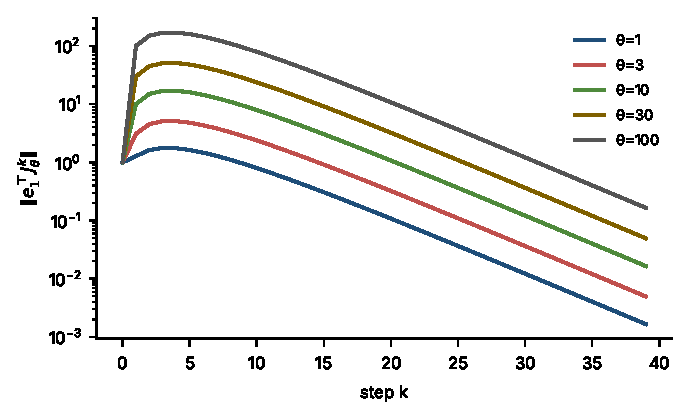
\includegraphics[width=0.6\textwidth]{figs/fig_blind.pdf}
\caption{Price-row transient gain of the spectral-blindness family $J_\theta$: eigenvalues $(0.8,0.7)$, one-step price variance 1 and stationary price variance 5 are the same for every $\theta$.}\label{fig:blind}
\end{figure}

Two clarifications prevent over-reading. First, the cohort economy of Section~\ref{sec:model} is itself non-normal, yet its price output does not amplify (Lemma~\ref{lem:cm}). Large weighted gains can be manufactured by output weights alone: with $C_w=(1,160)$, a price-and-memory functional peaks at $160.003$ at $t=0$, which is the static weight, not dynamic growth (Appendix~\ref{app:coordw}). Second, in a network of $M$ identical cohort economies coupled by symmetric nonnegative cross-impact, the coupled operator stays symmetric in the coordinates of Lemma~\ref{lem:cm}; with cross-impact $0.05$, the spectral radius rises from $0.822$ ($M=1$) to $0.973$ ($M=10$) while the Kreiss constant stays at one, as it must for a stable symmetric operator (\texttt{recompute\_oct20.py}). Non-normality is necessary for transient amplification of the price, not sufficient; where amplification comes from is the subject of the companion paper.
